\section{Modelado y perfiles de hogares}
\subsection{Disección experimental}
La unidad de análisis es el hogar (12.726 hogares, 63 predictores). La variable objetivo es \texttt{p0} (pobreza por ingreso, 37,9\,\% sin ponderar y 37,8\,\% ponderada). Se excluyen \texttt{p0}, \texttt{pext0}, \texttt{factor} y \texttt{folio} de los predictores, y no se usa ninguna variable de ingreso (lista negra documentada). La validación es \emph{agrupada por UPM}: el grupo es el segmento de muestreo (los dos primeros bloques del \texttt{folio}, 1.088 grupos), de modo que ningún segmento aparece a la vez en entrenamiento y prueba. Se usa \texttt{StratifiedGroupKFold} de 5 pliegues con semilla 42 y una partición única 80/20 (10.180 / 2.546 hogares, 870 / 218 UPM) que se toca una sola vez, al final. Todo el preprocesamiento (one-hot con \texttt{min\_frequency=20} para las 50 variables categóricas y estandarización de las 13 numéricas cuando aplica) va dentro del \texttt{Pipeline} y se ajusta solo con el entrenamiento de cada pliegue. El desbalance moderado (38\,\% de clase positiva) se maneja con \texttt{class\_weight="balanced"} en lugar de remuestreo. Las métricas de validación cruzada y de prueba se calculan sin ponderar; se reporta además el AUC ponderado con \texttt{factor}.

\subsection{Comparación de modelos}\label{sec:comparacion}
Se compararon cuatro familias de modelos, cada una con y sin pesos de clase balanceados (8 variantes en total), con búsqueda de hiperparámetros por validación agrupada de 3 pliegues dentro del entrenamiento. La Tabla~\ref{tab:modelos} resume el desempeño y la Figura~\ref{fig:roc} muestra las curvas ROC y Precision-Recall del modelo elegido en el conjunto de prueba.

\begin{table}[ht]\centering\caption{Desempeño de los modelos (AUC de validación cruzada agrupada y de prueba; métricas de prueba con umbral 0,5 salvo indicación).}\label{tab:modelos}
\begin{tabular}{lcccc}\toprule
Modelo & AUC CV & AUC prueba & Recall & Precisión \\\midrule
Regresión logística (sin pesos) & 0,851 & 0,831 & 0,62 & 0,71 \\
Regresión logística (balanceada) & 0,851 & 0,831 & 0,75 & 0,66 \\
Árbol de decisión (sin pesos) & 0,813 & 0,796 & 0,64 & 0,66 \\
Árbol de decisión (balanceado) & 0,813 & 0,800 & 0,73 & 0,60 \\
Random Forest (sin pesos) & 0,850 & 0,835 & 0,62 & 0,72 \\
Random Forest (balanceado) & 0,850 & 0,832 & 0,72 & 0,65 \\
\textbf{Gradient Boosting (balanceado, elegido)} & \textbf{0,856} & \textbf{0,838} & \textbf{0,75} & \textbf{0,63} \\
Gradient Boosting (sin pesos) & 0,856 & 0,837 & 0,64 & 0,71 \\\bottomrule\end{tabular}\end{table}

\begin{figure}[ht]\centering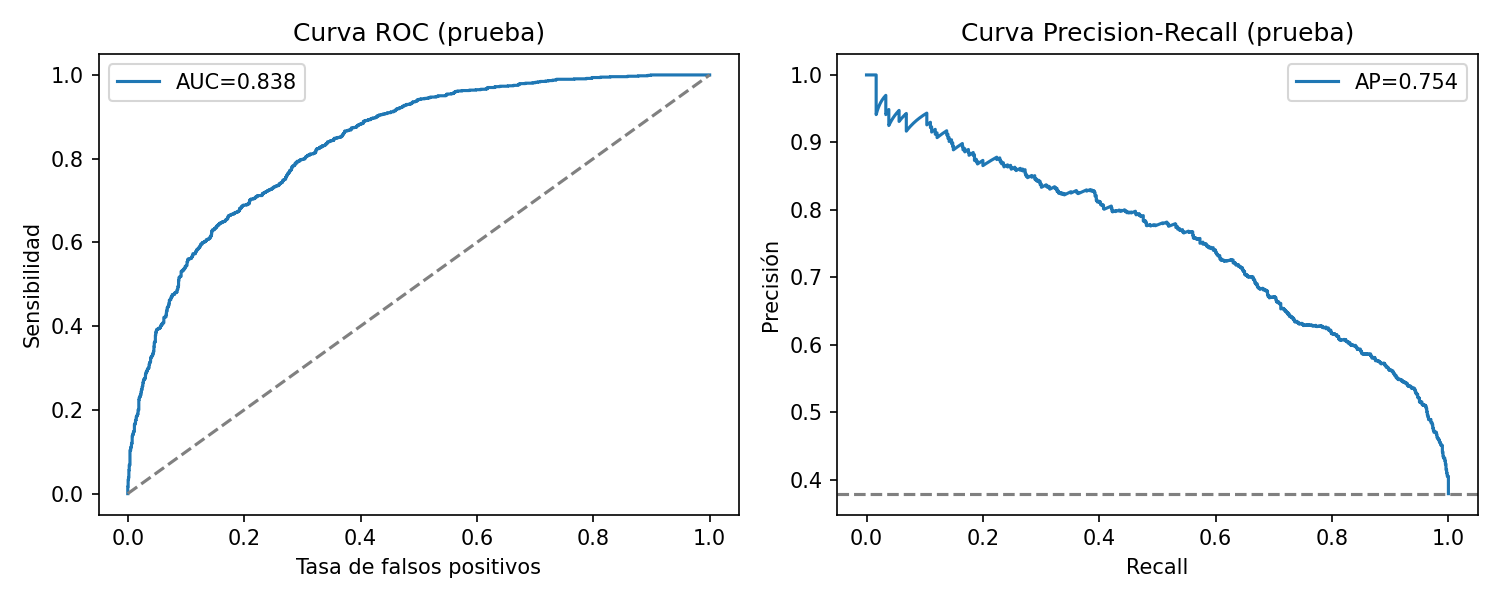
\includegraphics[width=.85\textwidth]{resultados/figuras/01_roc_pr.png}
\caption{Curvas ROC y Precision-Recall del modelo elegido (Gradient Boosting balanceado) en el conjunto de prueba.}\label{fig:roc}\end{figure}

Los ensambles mejoran apenas unos puntos de AUC sobre la regresión logística (0,856 frente a 0,851 en CV), lo que indica que la pobreza por ingreso se explica en gran parte de forma casi lineal a partir de las características del hogar. El árbol de decisión solo es claramente inferior (AUC CV 0,813).

\subsection{Modelo y umbral elegidos}
Se eligió el \textbf{Gradient Boosting con pesos de clase balanceados} (\texttt{HistGradientBoostingClassifier}, mejor configuración: \texttt{learning\_rate=0,1}, \texttt{max\_leaf\_nodes=8}, \texttt{min\_samples\_leaf=20}, \texttt{l2\_regularization=0}, parada temprana), por su mayor AUC de validación cruzada agrupada (0,856). En el conjunto de prueba alcanza AUC 0,838 (0,845 ponderado), AUC-PR 0,66 y Brier 0,164. El umbral de decisión se fijó en \textbf{0,488} maximizando el F1 en el entrenamiento; en prueba detecta 737 de 965 hogares pobres (recall 0,75) marcando 436 de 1.581 no pobres (precisión 0,63). Las predicciones fuera de pliegue sobre los 12.726 hogares dan un AUC de 0,856.

La columna \texttt{prob\_pobreza} exportada está \textbf{calibrada} con regresión isotónica sobre las predicciones fuera de pliegue: su media es 0,379, prácticamente igual a la tasa real de pobreza (0,379 sin ponderar y 0,378 ponderada), frente a 0,451 de la escala cruda inflada por los pesos balanceados. La calibración es monótona, por lo que no altera el AUC ni el orden de los hogares; la clasificación se hizo con la puntuación cruda y el umbral 0,488 antes de calibrar. La Figura~\ref{fig:calibracion} muestra la calibración por deciles.

\begin{figure}[ht]\centering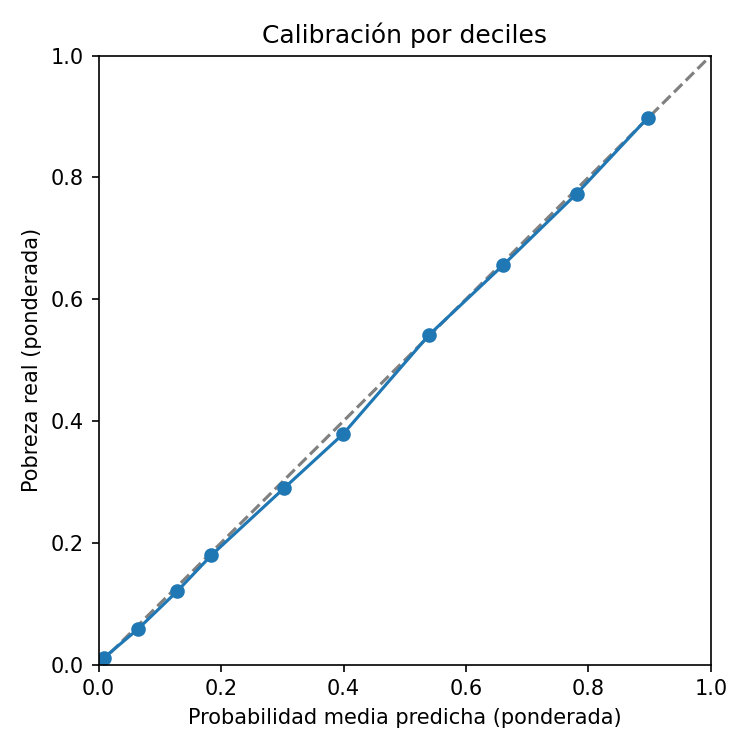
\includegraphics[width=.55\textwidth]{resultados/figuras/05_calibracion.png}
\caption{Calibración de \texttt{prob\_pobreza} por deciles (ponderada con \texttt{factor}).}\label{fig:calibracion}\end{figure}

\subsection{Variables influyentes}
La importancia por permutación sobre el conjunto de prueba (caída del AUC, 10 repeticiones) muestra un predictor dominante y varios secundarios (Figura~\ref{fig:importancia}): \texttt{tasa\_dependencia\_ocupados} (caída de 0,085, muy por encima del resto), \texttt{jefe\_tipo\_ocupacion} (0,025), \texttt{jefe\_grupo\_ocup} (0,017), \texttt{anios\_estudio\_prom\_15mas} (0,014), \texttt{depto} (0,013), \texttt{total\_activos\_hogar} (0,011), \texttt{prop\_menores\_14} (0,005) y \texttt{personas\_por\_dormitorio} (0,004). Los odds ratios de la regresión logística (con variables estandarizadas) confirman el sentido: más tamaño de hogar y más proporción de menores se asocian a mayor riesgo de pobreza; más miembros ocupados, más años de estudio y más activos del hogar se asocian a menor riesgo. La dependencia parcial (Figura~\ref{fig:pdp}) muestra relaciones monótonas en las variables numéricas más influyentes.

\begin{figure}[ht]\centering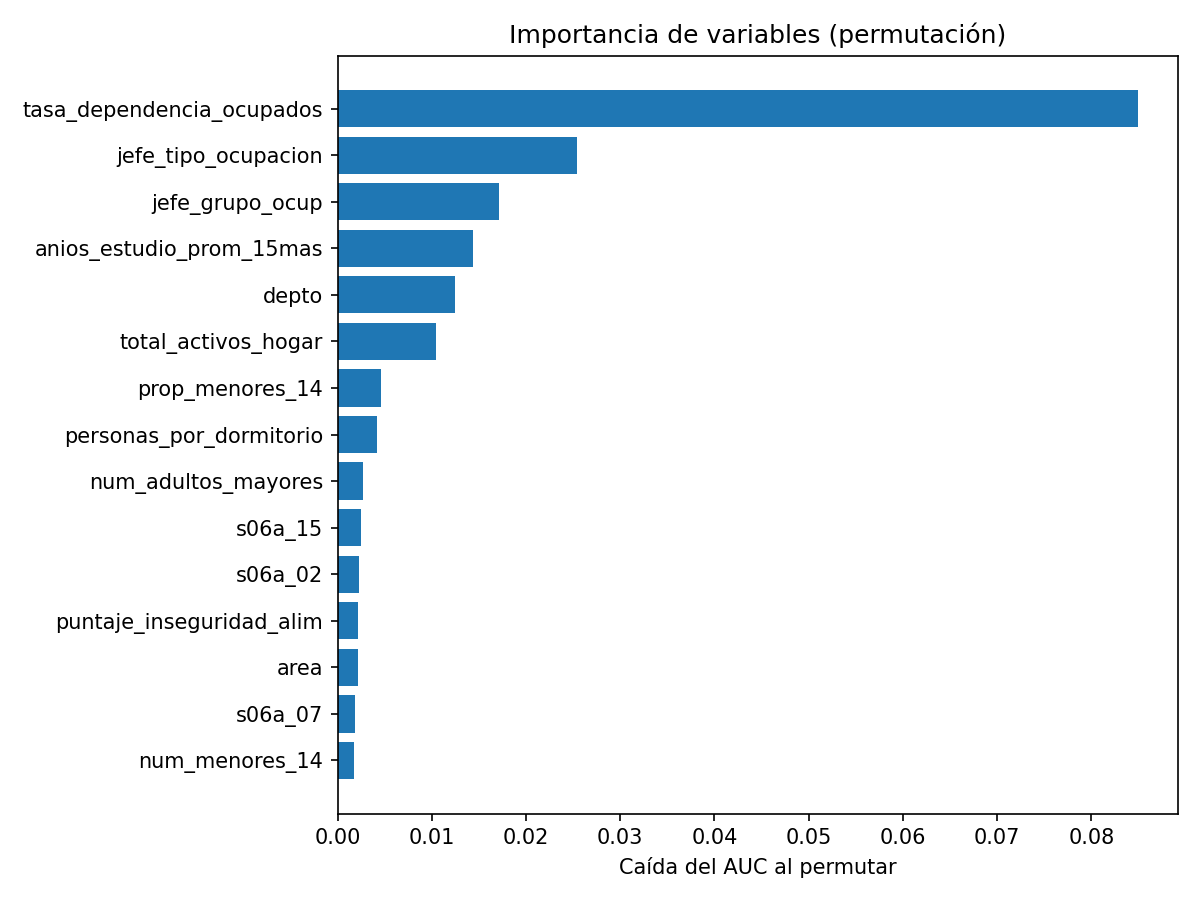
\includegraphics[width=.8\textwidth]{resultados/figuras/02_importancia.png}
\caption{Importancia de variables por permutación (caída del AUC en prueba).}\label{fig:importancia}\end{figure}

\begin{figure}[ht]\centering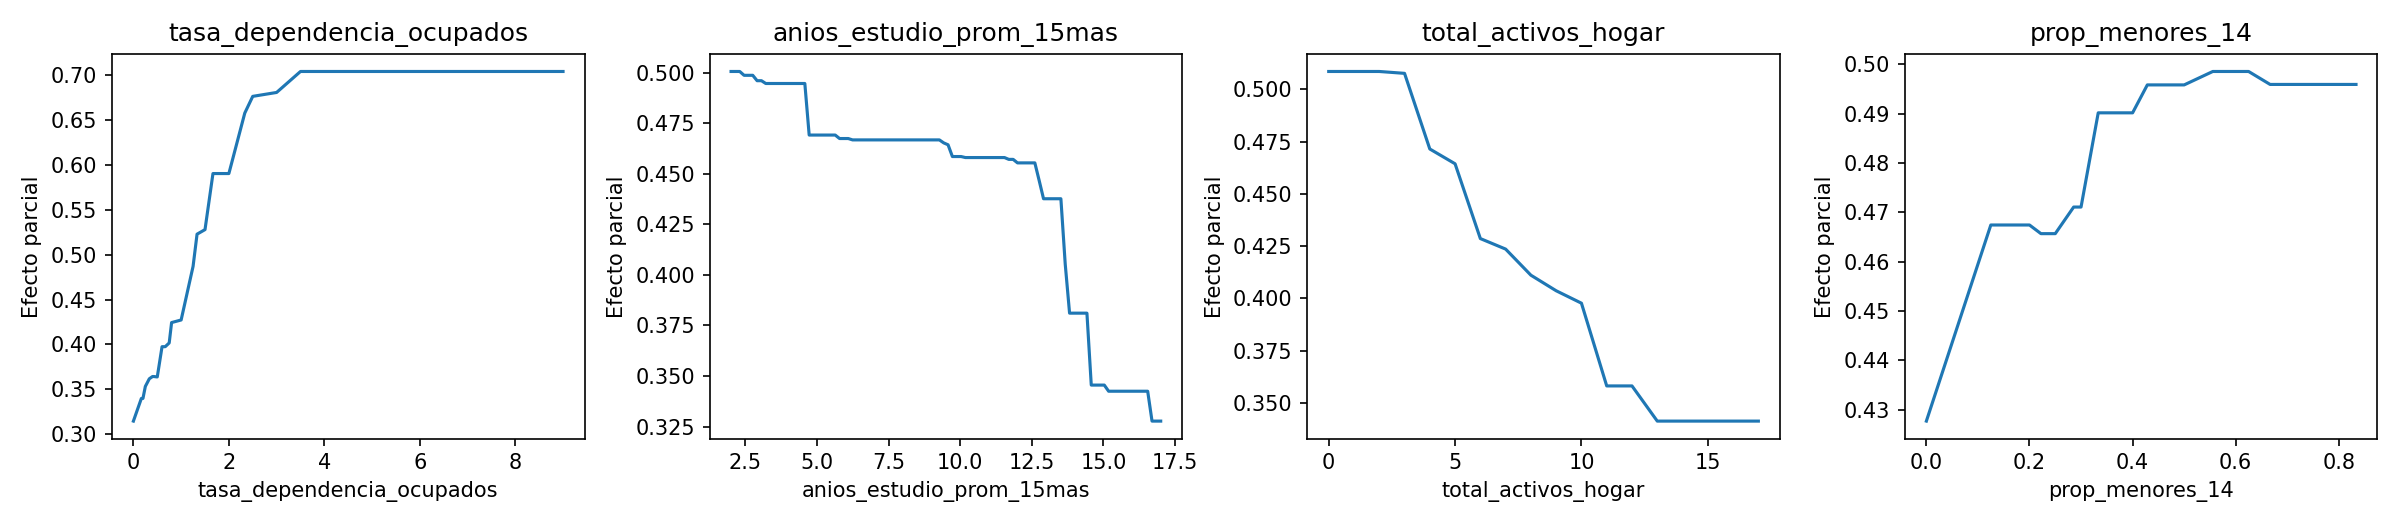
\includegraphics[width=.9\textwidth]{resultados/figuras/03_dependencia_parcial.png}
\caption{Dependencia parcial del modelo elegido para las variables numéricas más influyentes.}\label{fig:pdp}\end{figure}

\subsection{Sensibilidad y subgrupos}
La sensibilidad por grupos de variables (AUC de validación cruzada) muestra que ningún grupo es imprescindible: todos los predictores 0,855; sin inseguridad alimentaria 0,853; sin territorio (departamento y área) 0,852; sin ambos 0,850; sin equipamiento 0,855. En el conjunto de prueba el desempeño es muy similar entre Cochabamba (AUC 0,837, pobreza ponderada 37,1\,\%) y el resto del país (0,838), y entre el área urbana (0,835) y la rural (0,831, donde la pobreza ponderada es 48,2\,\% frente a 32,9\,\% en la urbana).

\subsection{Perfiles de hogares}
Se aplicó K-Means sobre 49 variables del hogar (estandarizadas, PCA al 90\,\% de varianza = 31 componentes). La selección de k se hizo con inercia, silueta, Calinski-Harabasz y Davies-Bouldin (Figura~\ref{fig:seleccionk}); k = 3 es estable entre semillas (ARI = 1,0) aunque la silueta es baja (0,10) y coincide poco con el agrupamiento jerárquico de Ward (ARI = 0,37). Por ello los perfiles se presentan como \textbf{tendencias, no grupos nítidos}. La Tabla~\ref{tab:perfiles} resume los tres perfiles (ponderados con \texttt{factor}) y las Figuras~\ref{fig:perfiles} y~\ref{fig:pca} los ilustran.

\begin{table}[ht]\centering\caption{Perfiles de hogares (clustering, ponderado con \texttt{factor}).}\label{tab:perfiles}
\begin{tabular}{lccc}\toprule
Perfil & \% hogares & Pobreza (\%) & Rasgos principales \\\midrule
0 · Hogares pequeños de adultos mayores & 24,7 & 44,8 & 1,9 personas; jefe de 62 años; 5,0 años de estudio; 3,6 bienes; 67\,\% rural \\
1 · Familias numerosas jóvenes & 31,7 & 57,8 & 4,3 personas; 37\,\% menores de 14; hacinamiento 53\,\%; jefe de 39,5 años; 9,5 años de estudio; 4,8 bienes \\
2 · Hogares urbanos con más estudios y bienes & 43,5 & 19,2 & 3,0 personas; jefe de 47,7 años; 13,4 años de estudio; 7,9 bienes; 94\,\% urbano; sin hacinamiento \\\bottomrule\end{tabular}\end{table}

\begin{figure}[ht]\centering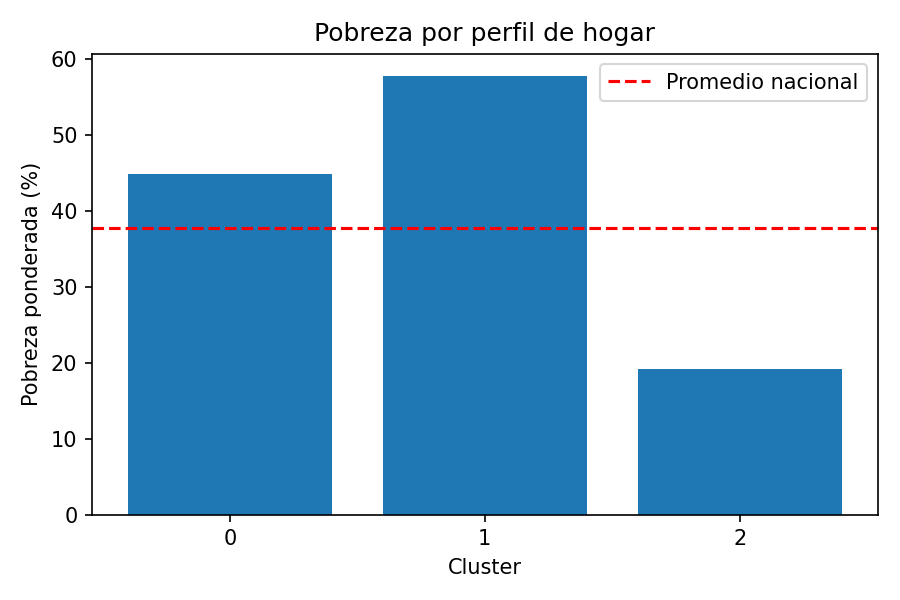
\includegraphics[width=.6\textwidth]{resultados/figuras/08_perfiles_pobreza.png}
\caption{Pobreza ponderada por perfil de hogar.}\label{fig:perfiles}\end{figure}

\begin{figure}[ht]\centering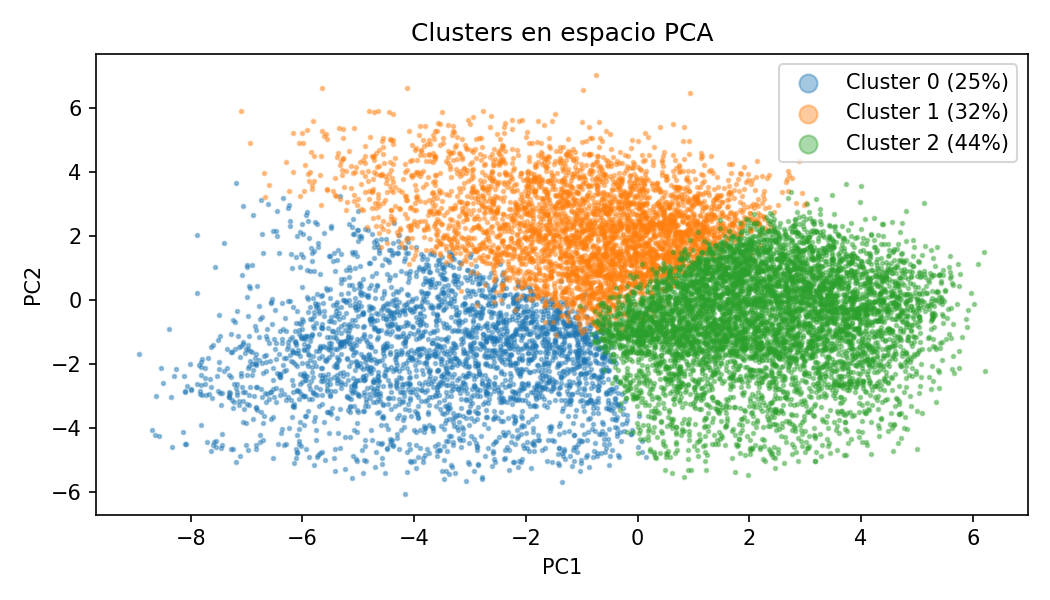
\includegraphics[width=.7\textwidth]{resultados/figuras/09_clusters_pca.png}
\caption{Perfiles en el espacio de los dos primeros componentes principales.}\label{fig:pca}\end{figure}

\begin{figure}[ht]\centering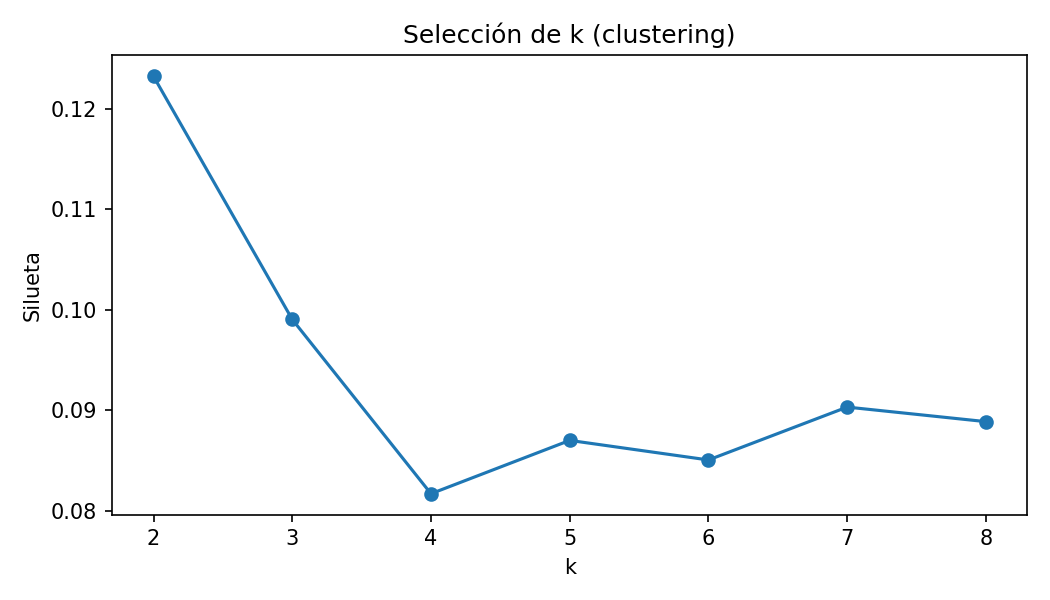
\includegraphics[width=.6\textwidth]{resultados/figuras/06_seleccion_k.png}
\caption{Selección de k para el clustering (silueta por k).}\label{fig:seleccionk}\end{figure}

\subsection{Reglas de asociación}
Como complemento no supervisado se minaron reglas de asociación sobre bienes y servicios del hogar (presencia y ausencia), con soporte mínimo del 5\,\%, confianza mínima del 55\,\% y lift mayor que 1,2, sobre la muestra sin ponderar. Las reglas más claras hacia la pobreza combinan la ausencia de bienes y servicios básicos: por ejemplo, \emph{``no posee cocina y no tiene baño con descarga de agua''} identifica hogares pobres con confianza del 65\,\% y lift 1,71; \emph{``sin agua por cañería de red y sin internet''} alcanza confianza del 60\,\% y lift 1,60. En sentido contrario, la posesión de bienes durables (refrigerador, lavadora, computadora, internet) y el jefe con estudios superiores se asocian con hogares no pobres (lift entre 1,2 y 1,3). El archivo \texttt{tablas/reglas\_asociacion.csv} contiene las 50 reglas seleccionadas (25 hacia \texttt{HOGAR\_POBRE} y 25 hacia \texttt{HOGAR\_NO\_POBRE}).

\subsection{Limitaciones}
La etiqueta de pobreza es monetaria (ingreso per cápita frente a la línea de pobreza del INE), por lo que está sujeta a subdeclaración del ingreso. Los datos son transversales: las asociaciones encontradas no implican causalidad. La inseguridad alimentaria puede ser consecuencia de la pobreza más que causa (su exclusión casi no cambia el AUC). Los perfiles de clustering son tendencias solapadas (silueta 0,10), no grupos nítidos. La calibración isotónica se ajustó y evaluó sobre las mismas predicciones fuera de pliegue, lo que la hace ligeramente optimista. Finalmente, \texttt{prob\_pobreza} es una estimación basada en características del hogar, no un diagnóstico.
